\documentclass[10pt,twocolumn]{article}
\usepackage{authblk}
\usepackage{tikz}
\usepackage{amsmath}
\usepackage[margin=.75in]{geometry}

\author{Daniel Leblanc}
\affil{Maseeh College of Engineering and Computer Science\\Portland State University\\Portland, OR}
\title{Simple Command-Line Artistic Toolset Implemented using OpenCV}
\date{June 12, 2013}

\begin{document}
\maketitle

\begin{abstract}
Numerous techniques have been developed for transforming photographs and other images into non-photorealistic representations.  Here we concentrate on implementing three of these techniques and how they can be combined to produce visually appealing results.  Edge sharpening with an extended difference of gaussian filter\cite{Winnemoeller:2012:XED} and painterly rendering with curved brush strokes \cite{Hertzmann:1998:PRC:280814.280951} combine to produce a painterly style image with clearer edges than the painterly rendering can produce when applied alone.  Both techniques also combine well with a salient preserving decolorization to produce a visually interesting grayscale image. 
\end{abstract}

\section{Introduction}
	\paragraph{}Many different methods for creating non-photorealistic renderings of images in various styles have been created.  We have implemented several of these styles and examined the results, as well as the results when multiple methods are combined.  The three techniques we have concentrated on are image sharpening using the extended difference of Gaussians by Holger Winnem{\"o}ller, Jan Eric Kyprianidis,  and Sven C. Olsen, \cite{ Winnemoeller:2012:XED}, painterly renderings with curved brush strokes by Aaron Hertzmann \cite{Hertzmann:1998:PRC:280814.280951}, and a salient preserving grayscale that is based on the works of Amy Gooch, Sven Olsen, Jack Tumblin, and Bruce Gooch, \cite{Gooch05color2gray:salience-preserving} and Chewu Lu, Li Xu and Jiaya Jia \cite{ lu:real-time}.
	\paragraph{} All techniques have been implemented using C++ and the OpenCV library.  The current design is a command-line interface that allows manipulation of the parameters used by the different techniques.

\section{Image Sharpening}
	\paragraph{} While the Winnem{\"o}ller paper demonstrates numerous powerful techniques that can be implemented using their extended difference of gaussian technique, we have implemented only their image sharpening here.  Other techniques such as crosshatching, flow extended difference of gaussian, and visual abstraction\cite{Winnemoeller:2012:XED} have been left as future excercises.
	\paragraph{} Image sharpening is accomplished using the XDoG filter as an adjusted image sharpening operator:
\begin{align}
	S_{\sigma, k, p}(x) = (1+p)\cdot G_{\sigma} (x) - p \cdot G_{k\sigma} (x)
\end{align}
The $G_{\sigma} (x)$ represents a gaussian blur with standard deviation $\sigma$ and $p$ is a user defined parameter that controls the degree of sharpening.  Best results were found with $p$ in the range $[10, 20]$ with higher values resulting in excessive noise and lower values being too similar to the original image.
	\paragraph{} Figures 2 and 3 are sharpened versions of our original image, figure 1, using parameters 10 and 20 respectively.  With $p = 10$ greater emphasis has been placed on the edges of the nose and the eyes compared to the original.  When $p=20$ that emphasis is enhanced even more, but a great deal of noise has also been introduced.  Minor difference that are almost invisible in the original image have been enhanced to the point of jarring contrast.

\begin{figure}
\centering
\begin{minipage}{0.15\textwidth}
\centering 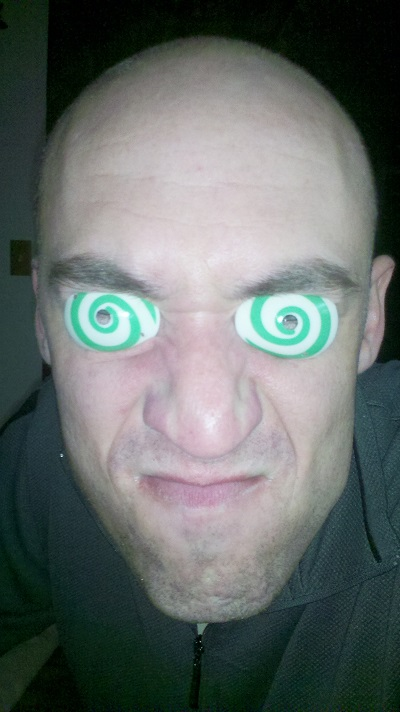
\includegraphics[width=\textwidth]{test3.jpg}
\caption{Original Image}
\end{minipage}
\begin{minipage}{0.15\textwidth}
\centering 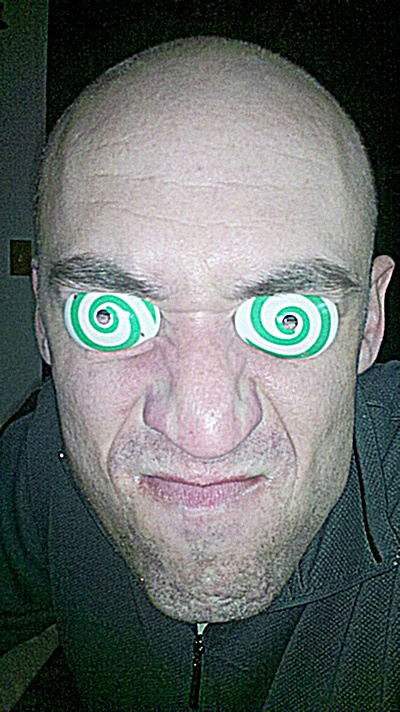
\includegraphics[width=\textwidth]{sharpface10.jpg}
\caption{$S_{\sigma, k, 10}(x)$}
\end{minipage}
\begin{minipage}{0.15\textwidth}
\centering \includegraphics[width=\textwidth]{sharpface.jpg}
\caption{ $S_{\sigma, k, 20}(x)$ }
\end{minipage}
\end{figure}

	\paragraph{} Interesting results can also be obtained by applying the sharpening to images other than photographs.  Figures 4, 5, and 6 show the same parameters applied to a digital painting.  When $p=20$ the noise is especially apparent in the mostly smooth background where artifacts have been introduced that disrupt the smooth gradient change, as shown in figure 7.

\begin{figure}
\centering
\begin{minipage}{0.15\textwidth}
\centering 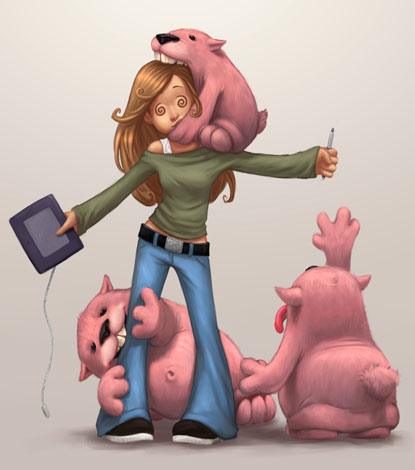
\includegraphics[width=\textwidth]{test2.jpg}
\caption{Original Image}
\end{minipage}
\begin{minipage}{0.15\textwidth}
\centering 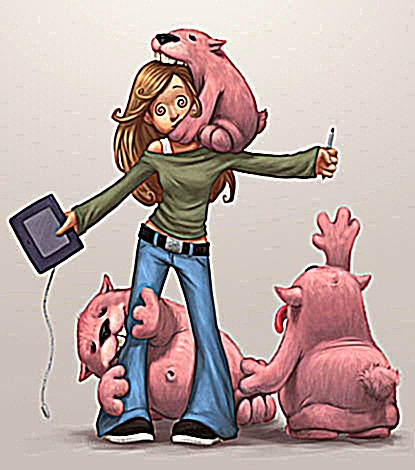
\includegraphics[width=\textwidth]{sharp10.jpg}
\caption{$S_{\sigma, k, 10}(x)$}
\end{minipage}
\begin{minipage}{0.15\textwidth}
\centering 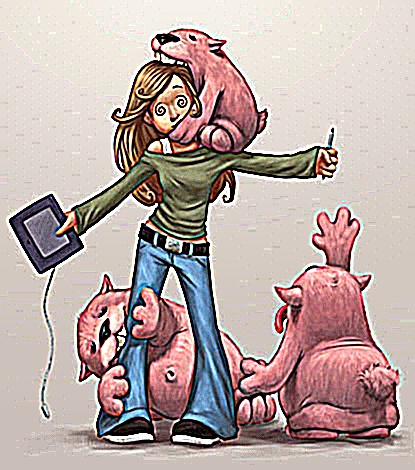
\includegraphics[width=\textwidth]{sharp20.jpg}
\caption{ $S_{\sigma, k, 20}(x)$ }
\end{minipage}
\end{figure}

\begin{figure}
\centering
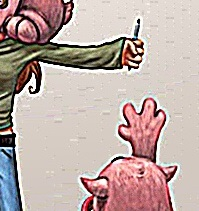
\includegraphics[width=0.45\textwidth]{sharpcrop.jpg}
\caption{Background artifacts}
\end{figure}

\section{Painterly Styles}
	\paragraph{} The goal of Hertzmann's technique \cite{Hertzmann:1998:PRC:280814.280951} is to produce an image with a hand-painted appearance from a photograph.  To do this a sequence of layers are created using lines of progressively smaller width.  In order to create lines that mimic what would be created by an artist, the lines are rendered as curves that are perpendicular to the direction of gradient change.  The lines are also applied in a random order to remove the influence of the sequence they are generated in.  Where strokes are placed is determined by the magnitude of the average difference between the existing canvas and a gaussian blur of the original image.  The canvas begins as an inverse of the final image to maximize the area covered by the first layer.  Subsequent layers concentrates on minor details and edges since areas lacking fine detail have already been covered by the earlier layers.

\begin{figure}
\centering
\centering 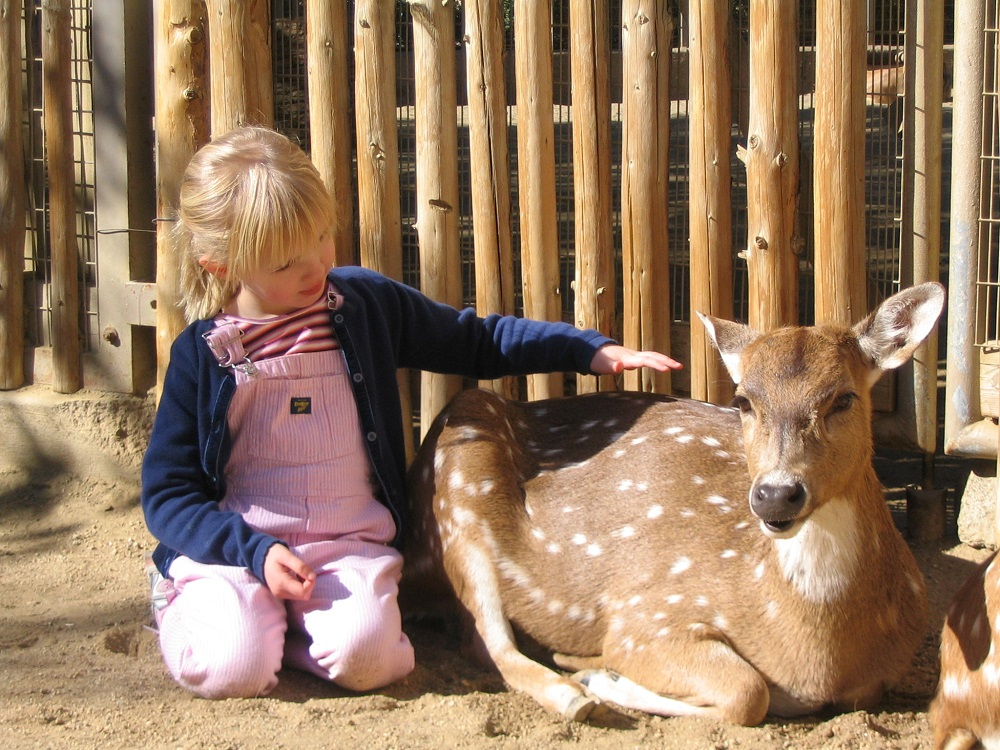
\includegraphics[width=0.45\textwidth]{test6.jpg}
\caption{Original Image}
\end{figure}
\begin{figure}
\centering 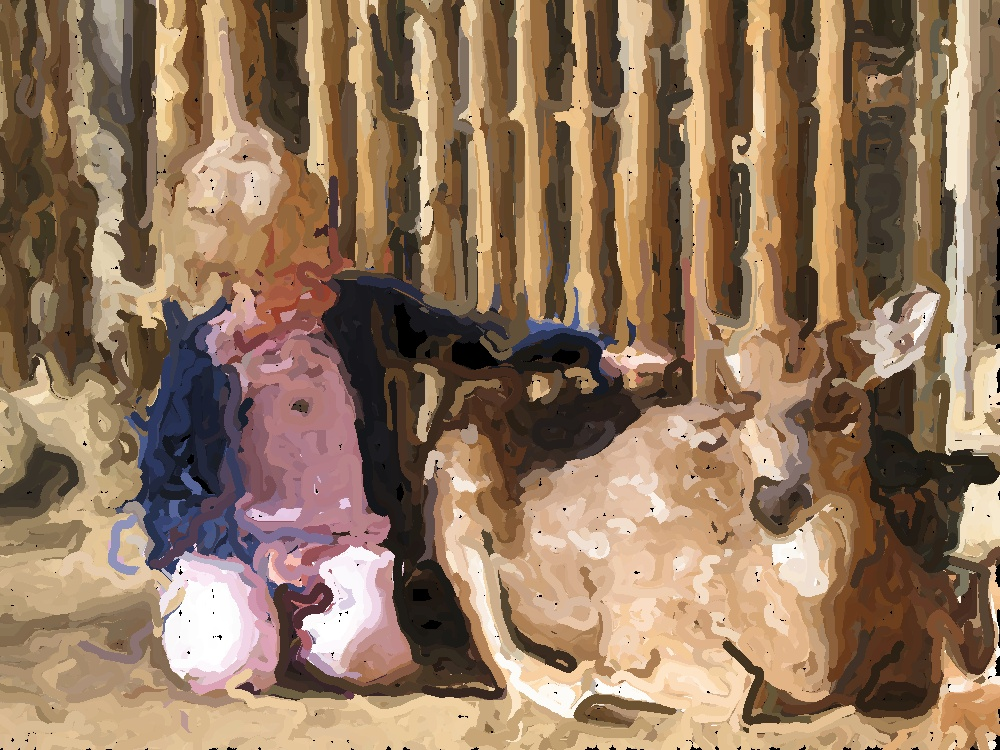
\includegraphics[width=0.45\textwidth]{paintDeer1.jpg}
\caption{After first layer}
\end{figure}
\begin{figure}
\centering 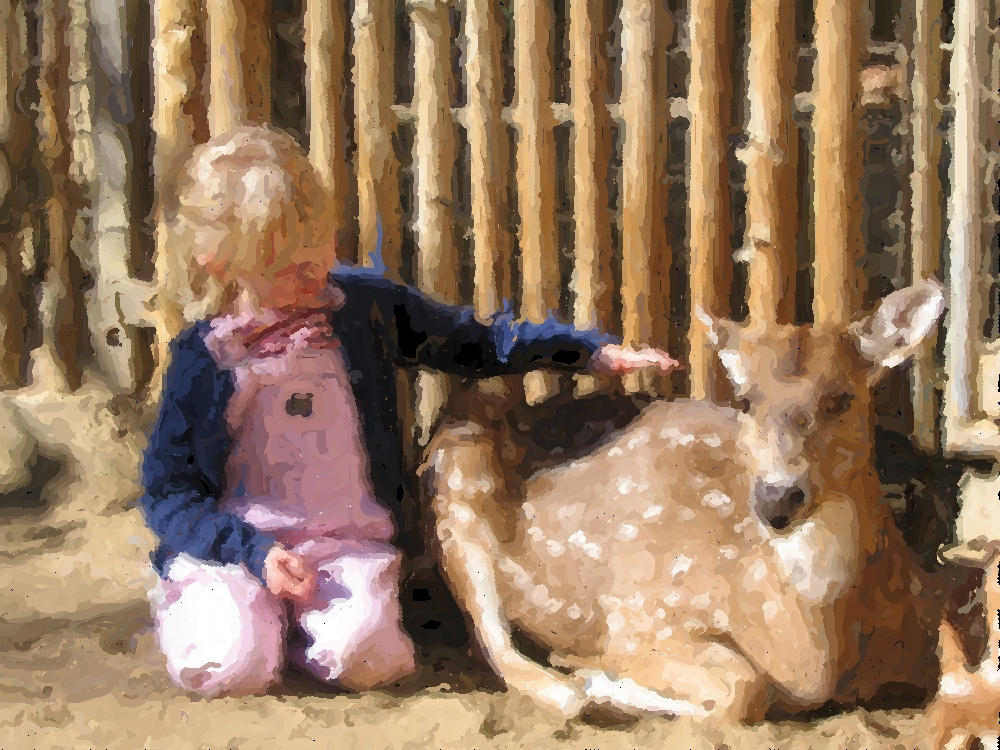
\includegraphics[width=0.45\textwidth]{paintDeer2.jpg}
\caption{After second layer}
\end{figure}
\begin{figure}
\centering 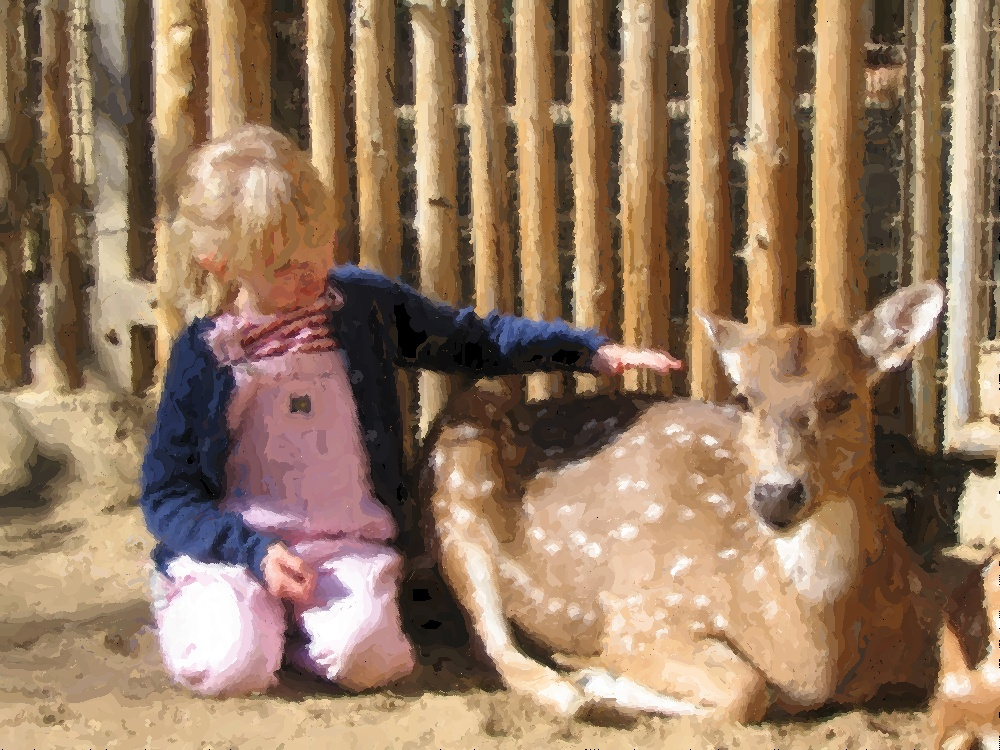
\includegraphics[width=0.45\textwidth]{paintDeer.jpg}
\caption{Final result}
\end{figure}

	\paragraph{} Figure 8 is the original image.  In figure 9 the first layer of brush strokes that define the larger areas have been placed.  Figures 10 and 11 show the next two layers as they refine the image details and produce the final result.  The current implementation occasionally fails to color every pixel, leaving some minor noise in the final result.  Figures 12 and 13 show the original image and the painterly image of the face we manipulated in the image sharpening section.

\begin{figure}
\centering
\begin{minipage}{0.24\textwidth}
\centering 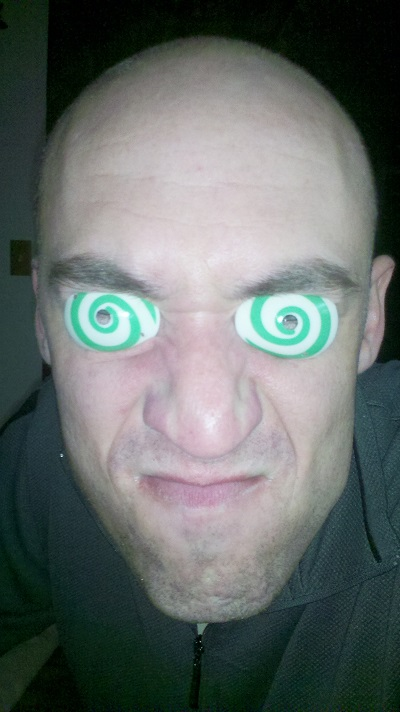
\includegraphics[width=\textwidth]{test3.jpg}
\caption{Original Image}
\end{minipage}
\begin{minipage}{0.24\textwidth}
\centering 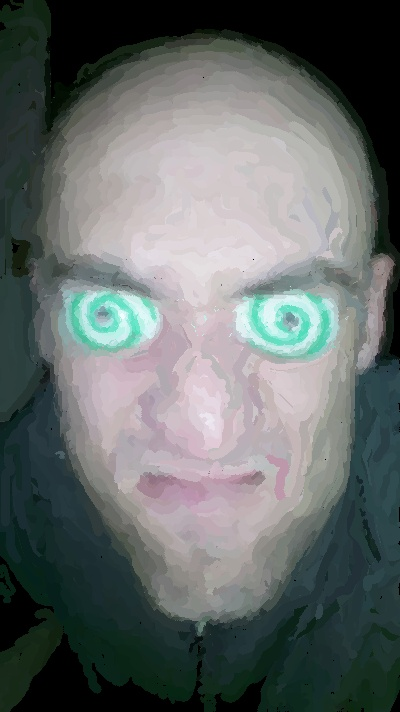
\includegraphics[width=\textwidth]{pfacebasic.jpg}
\caption{Rendered image}
\end{minipage}
\end{figure}

\section{Salient Preserving Grayscale}
	\paragraph{} The general goal of salience preserving decolorization is to preserve the contrast between different colors that have a similar luminance.  The Color2Gray method \cite{Gooch05color2gray:salience-preserving}, while extremely robust and producing excellent results, is much too slow to be applied to large images in real time.  The method presented in Real-time Constrast Preserving Decolorization\cite{lu:real-time}, while extremely fast, does not explain how they are determining the difference between colors.  The method we have implemented here uses the Color2Gray method for determining the difference between two colors and the real-time constrast preserving decolorization method for producing results extremely quickly.
	\paragraph{} In order to determine the color difference between two pixels, $s$ and $t$, the image is first converted from the $RGB$ to the $L^*a^*b^*$ color space.  Vectors $\vec{s_{ab}}$ and $\vec{t_{ab}}$ now represent the color of pixels $s$ and $t$.  We then calculate the angle between the two vectors to determine our color difference.\cite{Gooch05color2gray:salience-preserving}
	\paragraph{} There are two main reasons that the Color2Gray method is slow.  First, the number of pixel comparisons is extremely large, i.e. the number of pixels squared.  Second of all, the search space for the optimization has an infinite number of global minima\cite{Gooch05color2gray:salience-preserving}.  The real-time constrast preserving decolorization paper\cite{lu:real-time} addresses both of these issues to produce results in constant time.  To reduce the number of pixel comparisons a pool of $64^2$ pixel pairs is created, and the color difference is calculated for each one.  These pixel pairs are randomly chosen and rely on the redundancy inherent in color images to generate a reasonable representation of the possible color differences available.
	\paragraph{} To further reduce the number of comparisons needed the possible range of outputs is restricted to constant multiples in the RGB color space.  Three weights are produced such that:
\begin{align}
g &= w_1R + w_2G + w_3B \\
1 &= w_1 + w_2 + w_3
\end{align}
where $g$ represents the resultant grayscale value.  Restricting the sum of the weights to 1 ensures that the output is always in the correct range.  In order to further reduce the search space, the weights are restricted to multiples of $0.1$.  This reduces the total number of possible combinations to 66, which when combined with the small pixel pool allow for a complete search in just 30 milliseconds, regardless of the image size.
	\paragraph{} Figure 14 shows the OpenCV grayscale transformation next to the source image.  The strong contrast between the pink and the blue has been mostly lost with this result.  In figure 15 a strong contrast has been maintained between the two colors.  This has been obtained by reducing the impact of the red color channel on the grayscale output. While the final results are visually appealing for many images, they are not as consistently effective as what is produced using a larger search range.

\begin{figure}
\centering
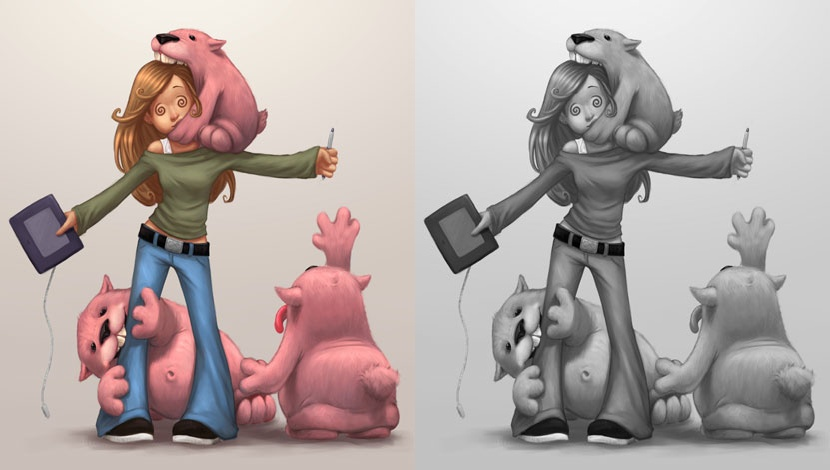
\includegraphics[width=0.45\textwidth]{greyC.jpg}
\caption{OpenCV grayscale}
\end{figure}
\begin{figure}
\centering
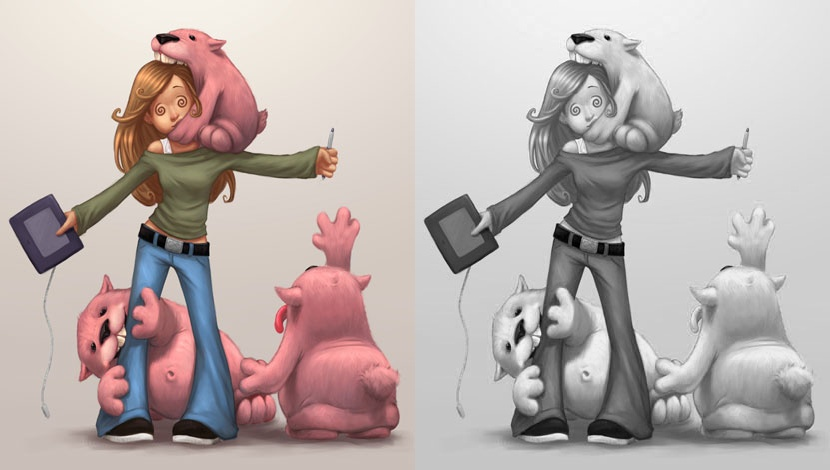
\includegraphics[width=0.45\textwidth]{greyL.jpg}
\caption{Contrast preserving grayscale}
\end{figure}

\section{Combined Results}
	\paragraph{} Visually appealing results were obtained by combining the techniques presented earlier in this paper.   The sharpened images produced with the extended difference of gaussian filter combined with the painterly renderings created more visually striking output than either produced alone.  
Figure 16 shows the original painterly style result on the left and the painterly style applied to the sharpened image from figure 2.  In figure 17, the left image is the painterly style applied to the sharpened image shown in figure 3, and the right image has had a median filter applied between the sharpening and the painterly rendering.

\begin{figure}
\centering
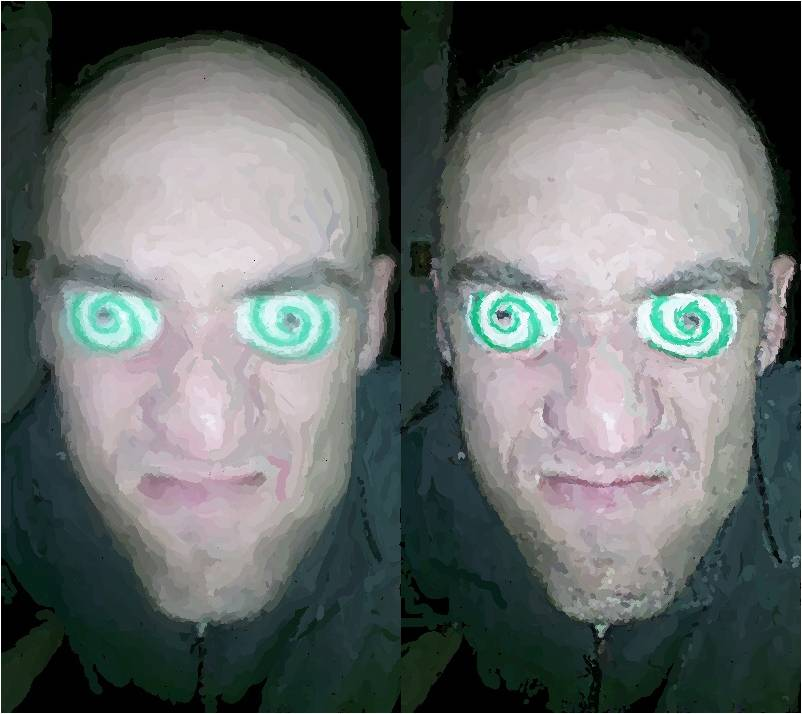
\includegraphics[width=0.45\textwidth]{sharppaint10.jpg}
\caption{Sharpened painterly style with $p=10$}
\end{figure}
\begin{figure}
\centering
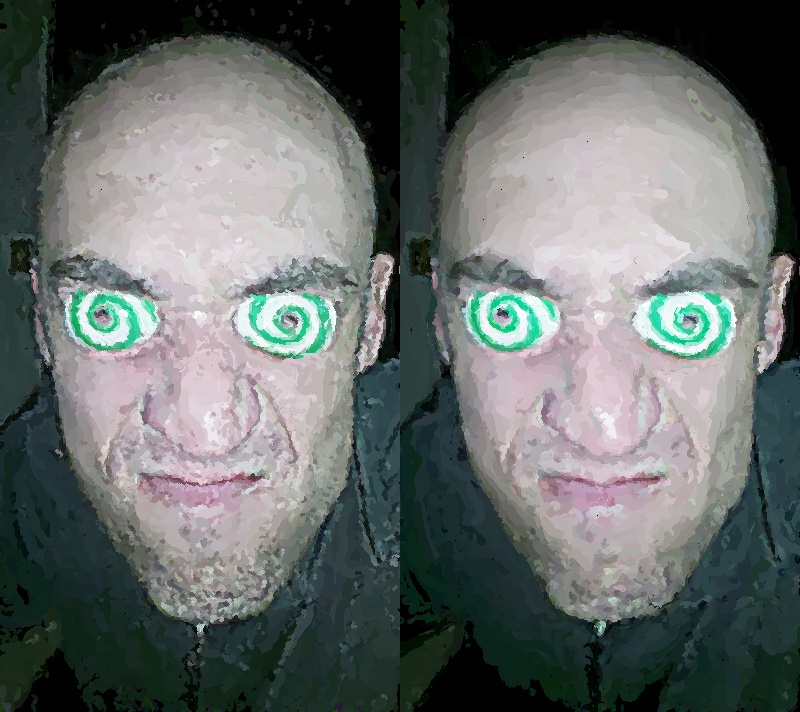
\includegraphics[width=0.45\textwidth]{medianpaint.jpg}
\caption{Sharpened painterly style with $p=20$ and the same image with a median filter}
\end{figure}

	\paragraph{} All three techniques presented in this paper are combined in figure 18.  In figure 19 the image from figure 8 has been sharpened, followed by a median filter and the painterly style.  Figure 20 shows that same image converted to grayscale using the technique presented.

\begin{figure}
\centering
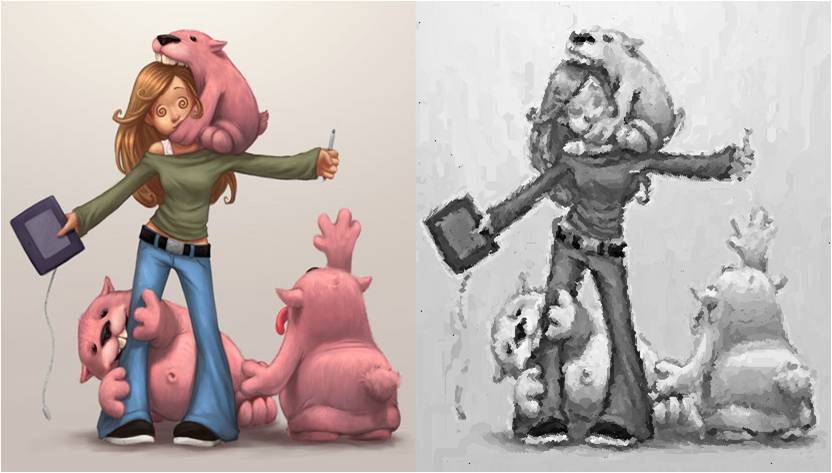
\includegraphics[width=0.45\textwidth]{all3.jpg}
\caption{A sharpened image followed by the painterly rendering and the grayscale conversion}
\end{figure}

\begin{figure}
\centering
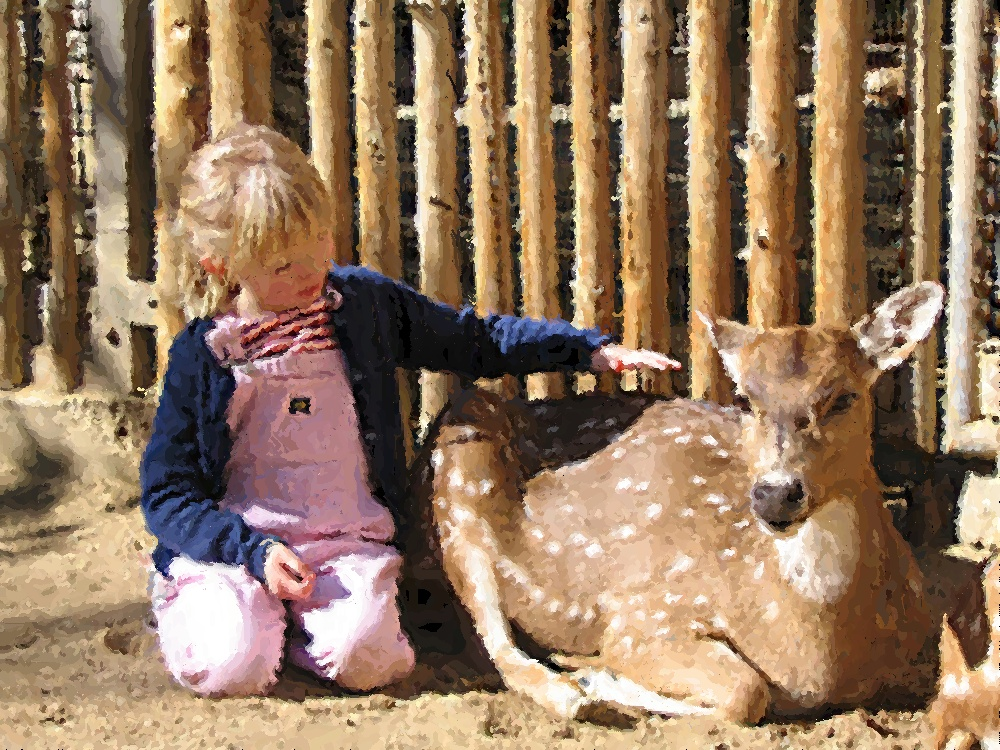
\includegraphics[width=0.45\textwidth]{smoothpaintdeer.jpg}
\caption{A sharpened image followed by a median filter and the painterly rendering}
\end{figure}
\begin{figure}
\centering
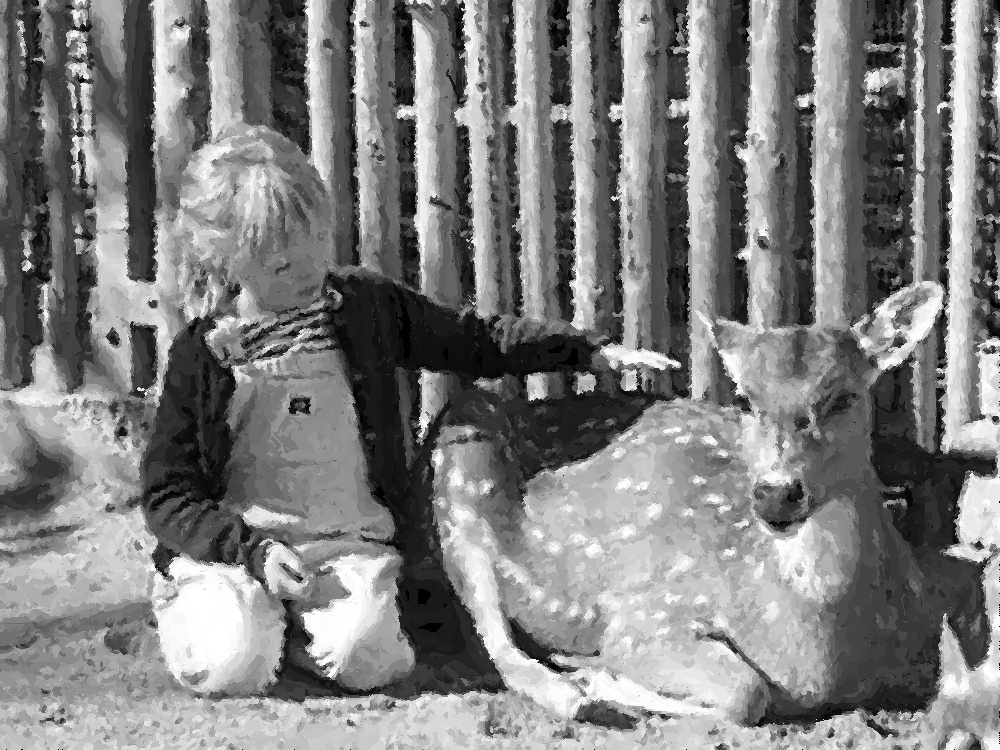
\includegraphics[width=0.45\textwidth]{grayPc.jpg}
\caption{Grayscale version of figure 19}
\end{figure}

\section{Conclusion and Future Work}
	\paragraph{} While many styles of non-photorealistic renderings are capable of producing visually appealing results when applied alone, combining multiple techniques can produce images that are subjectively better than the individual techniques can produce on their own.  Only a few different techniques are presented here and combinations of other techniques will likely produce even better results.
	\paragraph{} The current implementation is hampered by it's command line interface and future efforts will include building a more intuitive user interface that will allow for easier manipulation of the numerous parameters available.  The other obvious direction for future effort is expanding the array of tools that can be combined to produce the desired results.  The flow extended difference of gaussian technique offers potentially significant improvements over the current image sharpening.  Utilizing the GPU could also offer the ability to manipulate video using the painterly style in reasonable computation time.
	\paragraph{} The current grayscale conversion method also offers potential roads for improvement.  It may be possible to refine the size of the pixel pool further by concentrating on areas of interest.  This would allow for the range of possible weights to be expanded and potentially produce better results.

\nocite{*}
\bibliographystyle{plain}
\bibliography{citations}

\end{document}

